\documentclass[12pt,a4paper]{article}
\usepackage[top=25.4mm, bottom=25.4mm, left=19.1mm, right=19.1mm]{geometry}


\usepackage[latin2]{inputenc}
\usepackage{graphicx}
\graphicspath{ {./images/} }
\usepackage{ulem}
\usepackage{enumitem}
\usepackage{amsmath}
\usepackage[document]{ragged2e}

\setlength{\parindent}{4em}
\setlength{\parskip}{1em}
\usepackage{hyperref}

\usepackage{fancyhdr}
\pagestyle{fancy}
\fancyhf{}
\fancyhead[LO]{\textbf{\small IoT and Smart Analytics}\\
\text{\small A Program by IIITH and TalentSprint}}

\usepackage{xcolor}
\usepackage{lipsum}

\rhead{\begin{picture}(0,0) \put(-250,-2){
\includegraphics[width=9cm]{EXP_06_Images/ts-iisc-logo-pr.png}} \end{picture}}
\cfoot{\thepage}


\begin{document}

\begin{center}
\textbf{\large \\EXPERIMENT 25 }\\[6pt]
IoT through MQTT in ThingSpeak Cloud
\end{center}

\textbf{\large LEARNING OBJECTIVES:}\\[3pt]
At the end of this experiment, participants will be able to:\vspace{-6mm}\begin{enumerate}
 \setlength\itemsep{-0.3em}
\item  Create a ThingSpeak Account and a Channel for data Storage
\item  Use Thingspeak Cloud for IoT through MQTT Protocol
\item Retrieving data from ThingSpeak Cloud
\end{enumerate}

\textbf{\large APPARATUS REQUIRED:}\\
\vspace{-3mm}
\begin{enumerate}
 \setlength\itemsep{-0.3em}
\item ESP32-2-pcs 
\item USB cable-1pcs
\item Breadboard-2pcs
\item Power Adapter-1pcs 
\item DC-DC Voltage Converter Power Supply Module-1cs
\item Internet Connection
\item Jumper Wires
\end{enumerate}

\begin{justify}
\textbf{\large THEORY}\\[3pt]
Figure1. below shows the overview of the process involved in this experiment and in general. ThingSpeak MQTT Broker is used, where data from a sensor integrated with ESP 32 can be published. Another ESP32 is used for subscription and data can be displayed and based on the certain condition the same data can be used for actuation as well. Here we are going to use ESP32 as Publisher and Subscriber client but it could be any device that supports the MQTT protocol.


\begin{center} 
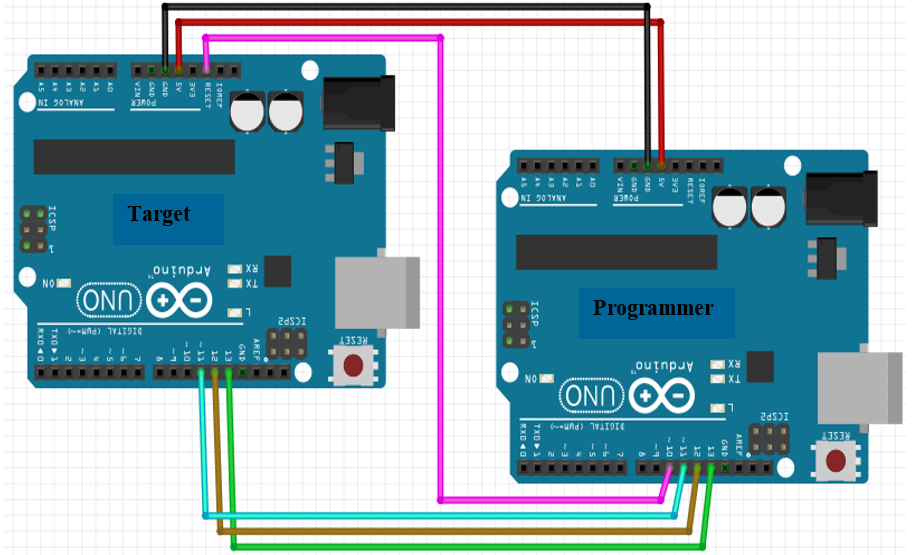
\includegraphics[scale=0.75]{EXP_25_Images/fig1.png}
\end{center}
\vspace{-10mm}
\begin{center} {Figure 1.Overview of the process}\end{center}



\noindent \textbf{\large PROCEDURE}\\[6pt]
\textbf{A)	Creating a ThingSpeak account \& a channel}\\
\vspace{-10mm}
\begin{enumerate}
 \setlength\itemsep{-0.3em}
\item  Open your Home Browser and go to the \href{https://thingspeak.com/}{URL} . A page similar to fig.2 given below is seen. Click on the icon highlighted in red for Signup/Login and another page as in fig.3 will display for filling your credentials.
\vspace{-5mm}
\begin{center} 
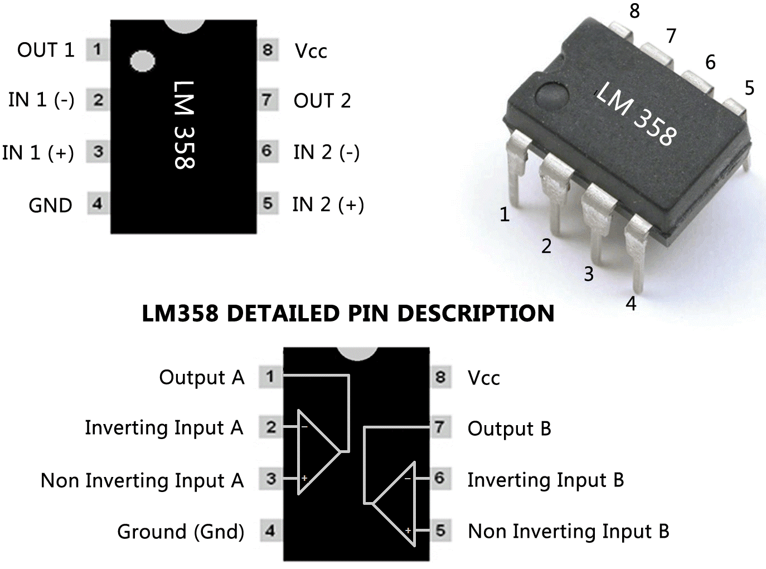
\includegraphics[scale=1]{EXP_25_Images/fig2.png}
\end{center}
\vspace{-10mm}
\begin{center} {Figure 2.Home page of ThingSpeak}\end{center}

\begin{center} 
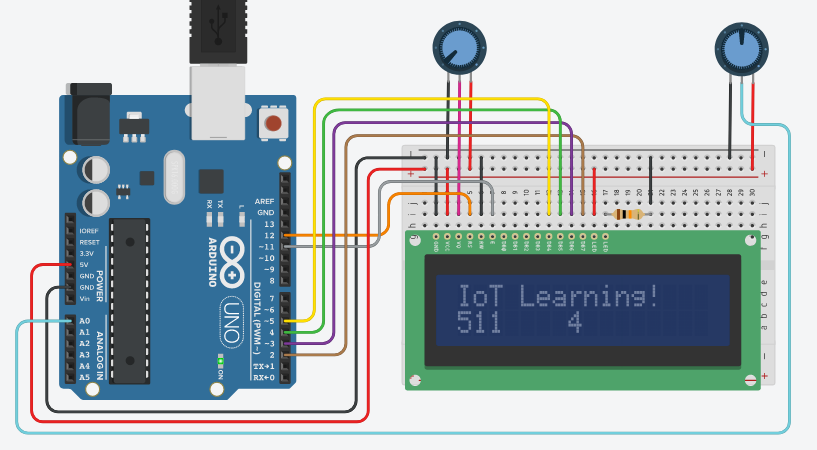
\includegraphics[scale=0.7]{EXP_25_Images/fig3.png}
\end{center}
\vspace{-10mm}
\begin{center} {Figure 3.Login page of ThingSpeak}\end{center}

\item  After successful login, we can see a page called Channels click New Channel as shown in fig.4 below.

\begin{center} 
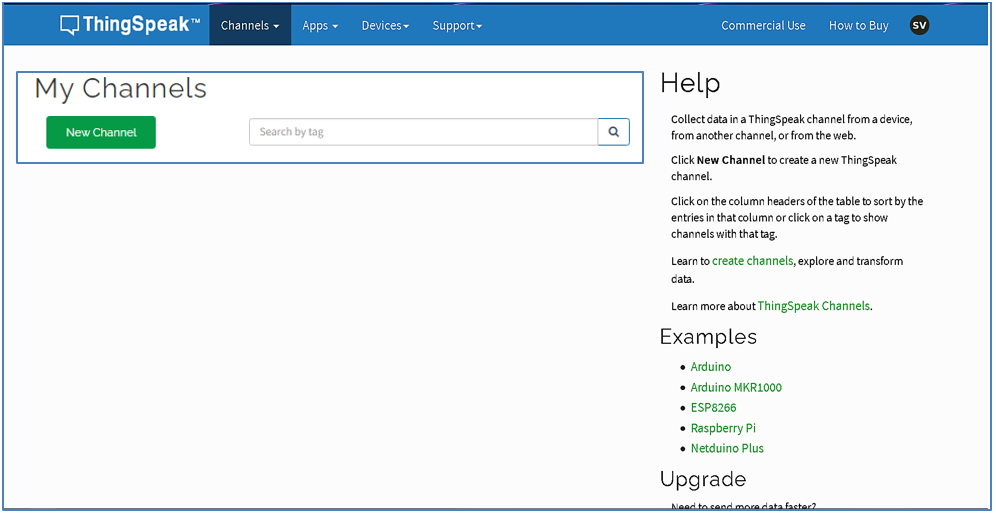
\includegraphics[scale=0.6]{EXP_25_Images/fig4.png}
\end{center}
\vspace{-10mm}
\begin{center} {Figure 4. Channel creation}\end{center}


\item Now Enter the Details as follows, as shown in fig.5, and then scroll down and press Save Channel.
\begin{enumerate}
    \item Name: Interfacing BME280 with ESP32
\item Description: Building a Mini Weather Station using BME280 and ESP32
\item Field 1: Temperature
\item Field 2: Relative Humidity
\item Field 3: Pressure
\item Field 4: Altitude\\[6pt]
\begin{center} 
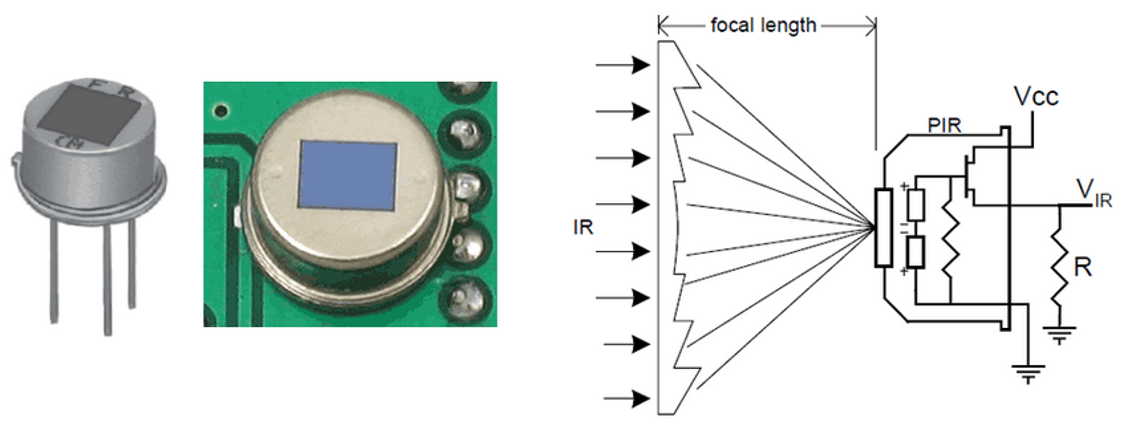
\includegraphics[scale=0.9]{EXP_25_Images/fig5.png}
\end{center}
\begin{center} {Figure 5. Field entry \& channel description}\end{center}
\end{enumerate}

\item After Pressing the Save Channel Button, you will be redirected to your Channel page, which has 4 Empty Graphs and your basic Channel Information. Click on the API keys Button as shown in fig.6 below

\begin{center} 
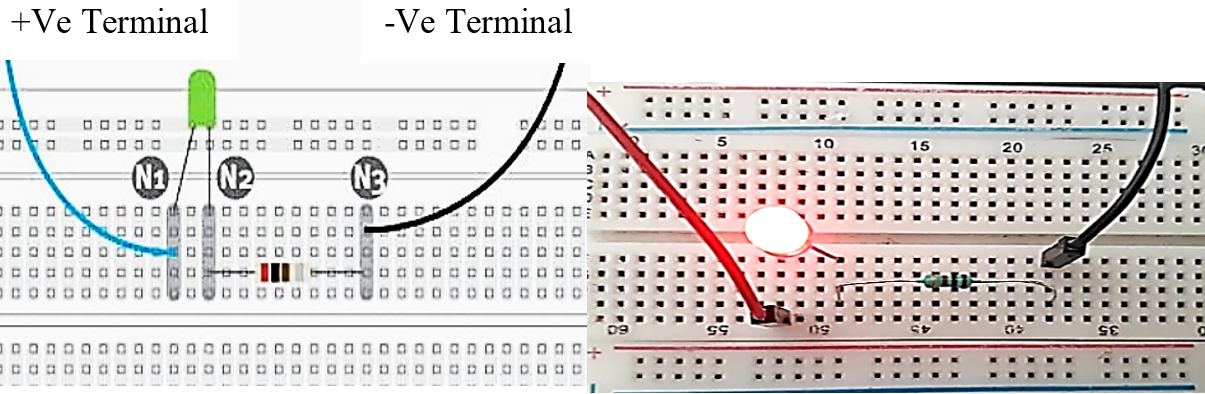
\includegraphics[scale=0.9]{EXP_25_Images/fig6.png}
\end{center}
\begin{center} {Figure 6.Channel page with graphs}\end{center}

\item There will be two API keys, one for writing and one for the read. Copy the Write API key \& save, as it will be used as an authentication token in our Arduino Code as shown in fig.7.

\begin{center} 
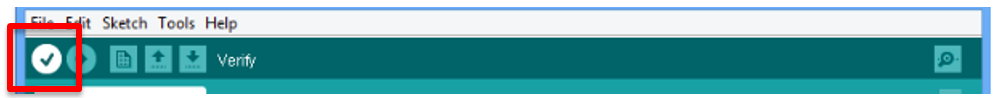
\includegraphics[scale=0.6]{EXP_25_Images/fig7.png}
\end{center}
\begin{center} {Figure 7.API key page }\end{center}
\end{enumerate}

\textbf{B)	Creating MQTT devices in ThingSpeak}\\
\vspace{-7mm}
\begin{enumerate}
\setlength\itemsep{-0.3em}
\item Once the channel is created to store the data, click on "Devices" and click on "MQTT", as shown in fig.8 below.
\item Click on \textbf{Add new device} and create a publishing device by filling in the \textbf{Device information}. Click on the test channel that is made for posting sensor data from \textbf{Authorize channels to access} list. Click on \textbf{Add channel} and tick \textbf{Allow Publish} as shown in fig.9 below.
\item After clicking on \textbf{Add Device} option, a window opens with MQTT publish credentials, as shown in fig.10 Make sure to download \& save the \textbf{Plain Text} file from the \textbf{Download Credentials} list. Click on \textbf{Done}.

\begin{center} 
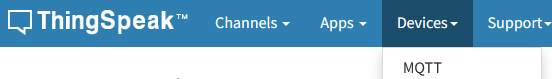
\includegraphics[scale=0.8]{EXP_25_Images/fig8.png}
\end{center}
\begin{center} {Figure 8.MQTT option }\end{center}

\begin{center} 
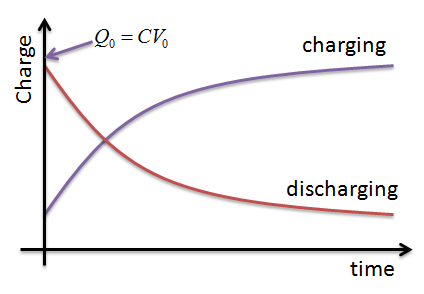
\includegraphics[scale=0.65]{EXP_25_Images/fig9.png}
\end{center}
\begin{center} {Figure 9. Creating publish device }\end{center}

\begin{center} 
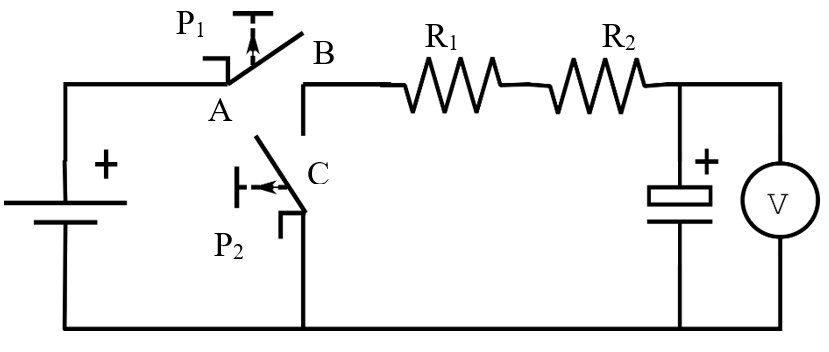
\includegraphics[scale=0.8]{EXP_25_Images/fig10.png}
\end{center}
\begin{center} {Figure 10. Creating publish device: getting credentials}\end{center}

After completing all the above 3 steps, we will see a page as given in fig.11 below:

\begin{center} 
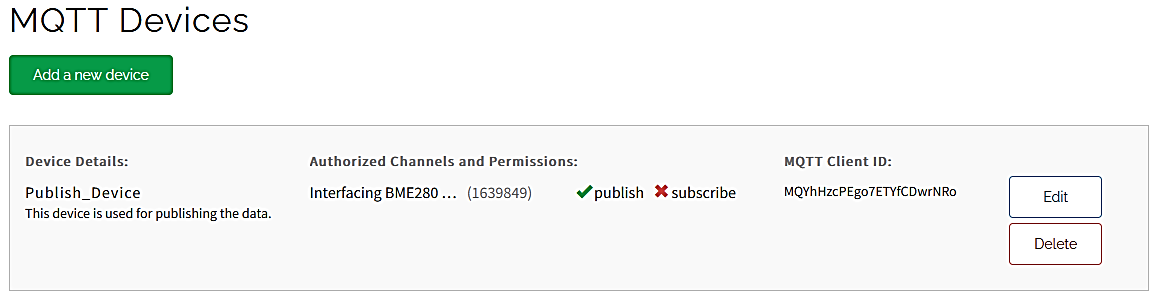
\includegraphics[scale=0.55]{EXP_25_Images/fig11.png}
\end{center}
\begin{center} {Figure 11. Publish device details}\end{center}
\item Click on Add a new device and follow similar steps to create an MQTT device for subscribing to data, as shown in fig.12, and make sure to store the credentials

\begin{center} 
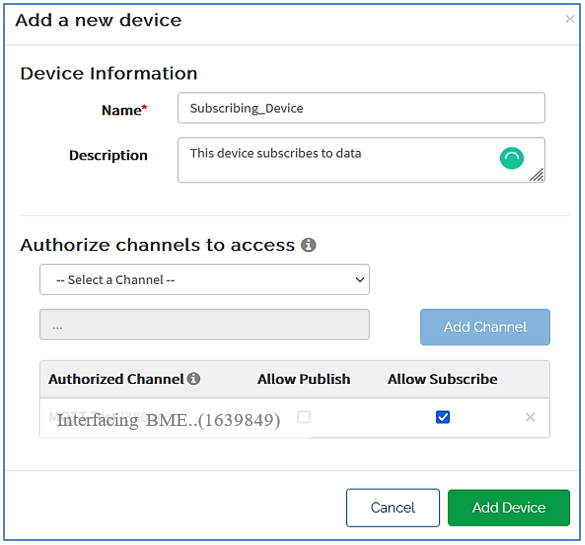
\includegraphics[scale=0.6]{EXP_25_Images/fig12.png}
\end{center}
\begin{center} {Figure 12. Creating subscribe device }\end{center}

\item Once the devices have been successfully created, the devices are as shown in fig.13.

\begin{center} 
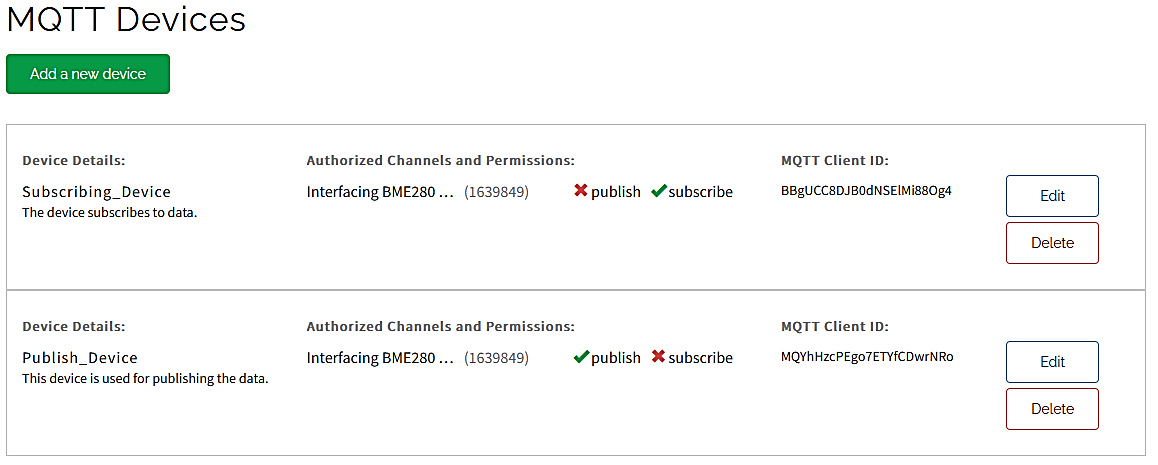
\includegraphics[scale=0.55]{EXP_25_Images/fig13.png}
\end{center}
\begin{center} {Figure 13. Both subscribe \& publish device details}\end{center}
\end{enumerate}

\noindent \textbf{C)	MQTT Publish-Subscribe in ThingSpeak with ESP32 as clients}\\[6pt]
Now we have both Publishing and Subscribing devices are ready to use for connecting with clients. In the first step, we will use one ESP32 as Publisher and send some data to the ThingSpeak cloud. The concept will remain the same and reading from any sensor integrated with ESP32 can be published.\par
\noindent In the second step, we will use another ESP32 as Subscriber and receive the data from ThingSpeak.\par

\noindent \textbf{Step 1: ESP32 as Publisher}\\
Upload the \textbf{'publisher.ino'}script in one ESP32 and open the serial monitor. We can see the data being sent to ThingSpeak. Similary, go to the channel created in ThingSpeak and click on \textbf{Private View}. We can see the data being uploaded in the graph. Here for simplicity, we have generated two random variable and send those data but the process remains same for any other data from any sensor as well. Don't forget to change the credentials according to your setting and use the credentials that we downloaded as a text file while creating the Publisher device.\par
\noindent \textbf{Note:} The Publisher ESP32 will keep running and sending the data to ThingSpeak.We have to remove the Publisher ESP32 from the PC/Laptop and power it via the DC-DC power module, before proceeding with the second step.

\noindent\textbf{Step 2: ESP32 as Subscriber}\\
Upload the \textbf{'subscriber.ino'} script in another ESP32 and open the serial monitor. We can see the data received from ThingSpeak. Don't forget to change the credentials according to your setting and use the credentials that we downloaded as a text file while creating the Subscriber device.


\noindent \textbf{D)	Retrieving BME280's Data From Thingspeak Cloud}\\[6pt]
The stored data can be retrieved in several ways out of which, a few of the possible ways are as described below:
\begin{enumerate}
    \item Extracting through API Methods: After clicking on the API section, a few links called API URLs are used to extract the data in any format, as shown in fig.14 below.
\item Another method would be extracting the whole data as a CSV File. After Clicking the Data Import/Export section the complete channel feed can be extracted as a CSV file.

\begin{center} 
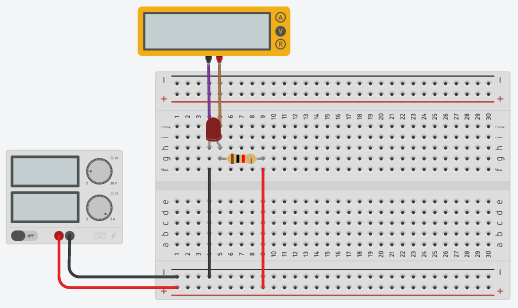
\includegraphics[scale=1]{EXP_25_Images/fig14.png}
\end{center}
\begin{center} {Figure 14. Data extraction through API }\end{center}
\end{enumerate}

\vspace{10pt}
\noindent \textbf{\large CONCEPT DRILL}\\[6pt]
Integrate BME280 or any other sensor with ESP32 and publish the data to ThingSpeak and subscribe those data again from ThingSpeak to other ESP32 and display on the serial monitor.

\end{justify}
\end{document}